\chapter{Implementation}\label{chapter:implementation}
This chapter explains how to set up a unikernel enabled kubernetes cluster with the required components. It also goes into detail of different implementation ideas that are also possible to extend this project or that were implemented by other parties. Implementation of the project consists of 4 parts.
\begin{enumerate}
\item Setting up the Kubernetes cluster
\item Implementing Virtual Kubelet
\item Setting up the edge environments
\item Developing unikernel applications
\end{enumerate}
\section{Setting up the Kubernetes Cluster}
The cloud provider for this thesis is Leibniz-Rechenzentrum, LRZ. They are using the OpenStack \cite{openstack} interface to provide computing services to their customers. While developing locally, microK8s was used to set up local ,short-lived, single node clusters. The testing was done on a kubernetes cluster set up by following the official documentation on their website. In that case, there is a Kubernetes master running on VM with 20 GB Disk , 9 GB RAM, 2 VCPUs and running Ubuntu-18.04. The kubernetes version is v1.16.3, which is the latest release at the time of writing. A secondary node is used for scaling experiments with the configuration similar to the master but with 4.5 GB RAM. The master node has a public IP so that devices can connect to it without a VPN. The pod network add-on used by the cluster is Cilium \cite{cilium}, as it's also being used in MicroK8s.

Another approach was to use Google Kubernetes Engine for setting up managed clusters. While they are easier to set up , connecting to them through non-Google-controlled devices is much more harder. 
\iffalse
Unikernels can be booted only in systems that either have a type-1 or a type-2 hypervisor. While they can be booted directly from BIOS on hardware, this does not give the flexibility required by cloud computing standards so a hypervisor is required to boot up and remove programs to achieve the desired state by the system.

Type-2 hypervisors run on a host operating system and they are easier to work with. If they provide an API, the host operating system can be used to develop programs to communicate with them. Given an example , a linux machine with virtualbox installed can boot up unikernel programs with terminal commands and no GUI is required. Then ,this terminal commands can be automated with a program that communicates with the internet.

For type-1 hypervisors, the task at hand is harder. There is no operating system involved and one has to work mostly with the API provided by the hypervisor itself. This calls for a program that either can be deployed to the hypervisor as a unikernel itself or for a virtual machine that can talk with the underlying hypervisor.
\fi



\section{Virtual Kubelet}
Virtual Kubelet\cite{virtual} is an open source project by Microsoft that aims to provide a programmable kubelet API interface to developers. It allows to deploy Kubernetes resource to different runtimes, transparent to the Kubernetes API. This project is currently a great candidate to deploy the unikernel solution proposed by this thesis. Virtual kubelet communicates with a custom pods provider to deploy resources. If the implementation of this thesis follows this approach, Virtual Kubelet will be forked and a new provider will be written for certain hypervisors to deploy unikernels. This also gives the opportunity to do a pull request to the project directly at the end of this thesis.

\begin{figure}[htpb]
  \centering
  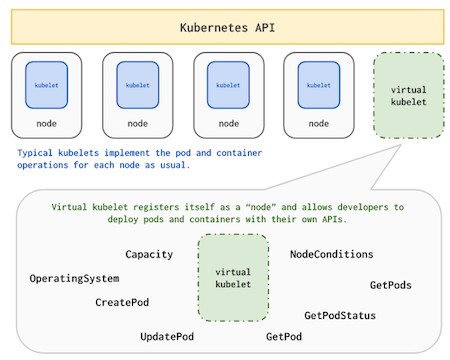
\includegraphics[width=0.8\textwidth]{figures/vk.png}
  \caption{Working principle of Virtual Kubelet \cite{virtual}} \label{fig:vk}
\end{figure}

Virtual Kubelet also opens possibilities to deploy unikernels to IoT devices through the Kubernetes API. Different virtual kubelet instances with different providers can work in parallel to deploy to target environments. This, again requires a receiver on the IoT device part. 
\subsection{Communication between cluster and device}
Kubernetes has a built-in service discovery. Deployed containers use hostnames instead of IPs to communicate between each other. Kubernetes runs a DNS server and maps those hostnames to IP addreses of individuals containers or mostly services. Unikernel deployments should also have the same functionality to work flawlessly with the rest of the kubernetes cluster. 

\subsection{Communication between kubernetes and hypervisor}
Kubernetes has a single endpoint for all the communication between the user and the cluster. This single endpoint should be aware of unikernel deployments so that it can schedule them accordingly. Kubernetes provides different ways to achieve this extensibility. First, it allows developers to create custom resource definitions such that they can be used together with other kubernetes resources. Second, kubernetes allow for deployment for different scheduler that can operate on specificly-tagged deployments. 


\section{Setting up edge environments}
\subsection{Type-2 Hypervisor}
\subsection{Type-1 Hypervisor}
\subsection{IoT Devices}

\iffalse
\section{Proposed Solution}

Before starting to implement unikernels to Kubernetes, a couple of proof of concept unikernel programs will be created. To create those programs, open-sourced unikernel solutions will be used. There are multiple projects with different approaches and different runtime environments. Next chapter explains more about those solutions. Selecting the most suitable one for the purpose of this thesis plays a crucial role because, it is out of scope for this thesis to develop a new unikernel solution just for Kubernetes. Once those programs are created, unikernel deployments will be added to kubernetes arsenal with the following steps:

1) A node with a type-2 hypervisor will be created. A custom program will be written that takes orders from a server and boot up unikernels according to parameters coming from the order. The custom program will run on the host operating system and there will be no kubernetes involvement.

2) A kubernetes cluster will be created and that custom program will be modified to communicate with kubernetes. Everytime a unikernel deployment is made, kubernetes will notify this program, and program will do the deployment.

3) Kubernetes DNS system will be integrated to the node with the type-2 hypervisor so they can communicate with other applications.

4) A node with a host operating system with type-1 hypervisor will be created. E.g. Xen hypervisor can also run on a host operating system. This node will be modified to communicate with the kubernetes cluster through the host operating system. 

5) A node without a host operating system with type-1 hypervisor will be created. This node should also run the custom program that communicates with the kubernetes cluster on the hypervisor and should also do the networking of unikernels between other kubernetes resources.This will be the final outcome of the thesis.

\begin{figure}[htpb]
  \centering
  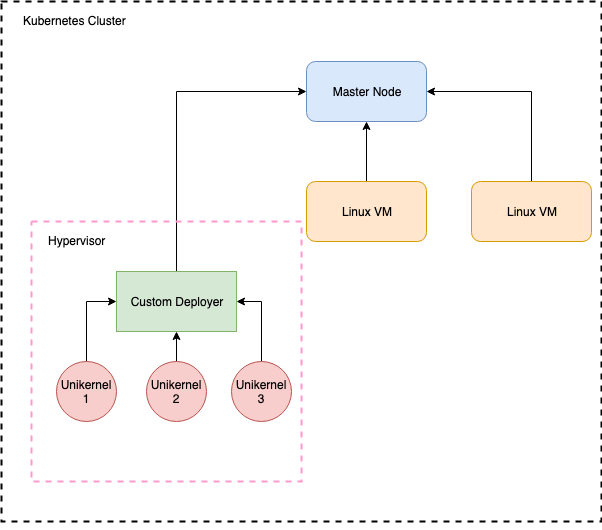
\includegraphics[width=0.8\textwidth]{figures/arch3.png}
  \caption{A kubernetes cluster with a only hypervisor enabled node for unikernel deployment} \label{fig:hypervisor}
\end{figure}


A scope of this project is not to come up with a new unikernel solution and it will use the ones already developed by the open-source community.It also won't compare application performance between docker containers and unikernels. It will although compare the deployment time between those.
\fi
\section{Developing Unikernel Applications}


